\documentclass[sigconf]{acmart}

\usepackage{booktabs} % For formal tables
\usepackage{graphicx}
\usepackage{url}
\usepackage{balance}

\usepackage{amsmath}
\usepackage{algorithm,algpseudocode,float}
\usepackage{amsmath}

% Copyright
%\setcopyright{none}
%\setcopyright{acmcopyright}
%\setcopyright{acmlicensed}
\setcopyright{rightsretained}
%\setcopyright{usgov}
%\setcopyright{usgovmixed}
%\setcopyright{cagov}
%\setcopyright{cagovmixed}




\begin{document}
\title{Scalability of Hybrid Sparse Matrix Dense Vector (SpMV) Multiplication}



\author{Brian Page}
\affiliation{%
  \institution{Univ. of Notre Dame}
  \streetaddress{326 Cushing Hall}
  \city{Notre Dame} 
  \state{Indiana} 
}
\email{bpage1@nd.edu}

\author{Peter Kogge}
\affiliation{%
  \institution{Univ. of Notre Dame}
  \streetaddress{326 Cushing Hall}
  \city{Notre Dame} 
  \state{Indiana}
}
\email{kogge@nd.edu}



% The default list of authors is too long for headers}
\renewcommand{\shortauthors}{}


\begin{abstract}
	TBD
\end{abstract}

%
% The code below should be generated by the tool at
% http://dl.acm.org/ccs.cfm
% Please copy and paste the code instead of the example below. 
%
\begin{CCSXML}
<ccs2012>
 <concept>
  <concept_id>10010520.10010553.10010562</concept_id>
  <concept_desc>Computer systems organization~Embedded systems</concept_desc>
  <concept_significance>500</concept_significance>
 </concept>
 <concept>
  <concept_id>10010520.10010575.10010755</concept_id>
  <concept_desc>Computer systems organization~Redundancy</concept_desc>
  <concept_significance>300</concept_significance>
 </concept>
 <concept>
  <concept_id>10010520.10010553.10010554</concept_id>
  <concept_desc>Computer systems organization~Robotics</concept_desc>
  <concept_significance>100</concept_significance>
 </concept>
 <concept>
  <concept_id>10003033.10003083.10003095</concept_id>
  <concept_desc>Networks~Network reliability</concept_desc>
  <concept_significance>100</concept_significance>
 </concept>
</ccs2012>  
\end{CCSXML}

\ccsdesc[500]{Computer systems organization~Embedded systems}
\ccsdesc[300]{Computer systems organization~Redundancy}
\ccsdesc{Computer systems organization~Robotics}
\ccsdesc[100]{Networks~Network reliability}


\keywords{multi-threading, parallel systems, mobile threads, memory architectures, performance, PGAS}


\maketitle

\section{Introduction}\label{sec:dspmv-intro}

The product of a sparse matrix and a dense vector (\textbf{SpMV}) is a key part of many codes from disparate areas. Numerically, it makes up the bulk of the High Performance Conjugate (HPCG) \cite{techbib:hpcg-snl-dongarra} code that has become an alternative to LINPACK for rating supercomputers.\footnote{http://www.hpcg-benchmark.org/} When the matrix operations are changed from product and add to a variety of other non-numeric functions that still form semi-rings, it becomes an essential part of many graph kernels \cite{bigdata:doi:10.1137/1.9780898719918}, and is a key function in the recently released GRAPHBLAS spec \cite{graphblas}. There has even been a novel prototype hardware system built around such sparse operations \cite{techbib:song-hpec}.

\begin{figure}\begin{centering}
		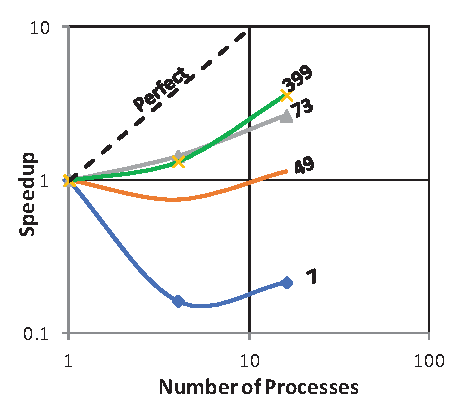
\includegraphics[scale=0.70]{figures/spmv-bylina-speedup.eps}
		\caption{Speedup from \cite{techbib:6933066} for 4 Sparse Matrices}
		\label{fig:spmv-bylina-speedup}
\end{centering}\end{figure}

Motivating the work presented here was an earlier study, \cite{techbib:6933066}, that looked at scaling of SpMV for a variety of matrices of varying sparsity from a well-known repository.\footnote{https://www.cise.ufl.edu/research/sparse/matrices/} What caught our interest was an observed significant dip in speedup (see Fig. \ref{fig:spmv-bylina-speedup} where the numbers on each line is the average non-zeros per row) that approached an order of magnitude  for the sparsest cases, and from which recovery was slow as the available compute resources increased. We have observed similar dips in other kernels and wanted to explore this phenomena more closely. 

Our specific goal was thus to duplicate the results, explore the cause of the dip, and extend the range of scaling, all as a precursor for developing better codes for these very sparse cases that would scale well to very large systems. However, in the process of performing this study, we found that the matrices used (all symmetric) were filed in the repository in a compressed lower form with only the lower diagonal half of non-zeros stored, and that even though the matrices were discussed in \cite{techbib:6933066} in terms of their actual uncompressed sparsity, the computational results seemed to have used only this lower half, which approximately halved the effective sparsity, and distorted the distribution of non-zeros  The work here has used the full version of these matrices.

In organization, Section \ref{sec:dspmv-analytic} discusses the generic algorithm and then builds a simple model for estimating performance, as well as prior work. Section \ref{sec:dspmv-implementation} discusses the code implemented here.Section \ref{sec:dspmv-evaluation} evaluates the results. Section \ref{sec:dspmv-conclusion} concludes.


\section{Related Work}\label{sec:dspmv-relatedwork}



\section{Implementation}\label{sec:dspmv-implementation}

- unlike Bylina et al's multinoda algorithm, which used BLACS to perform the data distribution amongst the cluster, as MKL to perfrom the multithreaded SpMV on each cluster node, a hybrid distrbuted SpMV was designed as a single stand alone entity. 
	- control over all MPI and OpenMP operations, including thread and process affinity, resource overscheduling, etc.
	- does not require software licensing
	- can be tailored to cluster size and node hoardware architecture
	
- the application was written in c++, compiled with openmpi with passthrough to the g++ compiler
	- compiled with openmp 
	- optimization level 3
	
- Careful attention was paid to the MPI communication structure such that it would emulate the behavior produced by the BLACS routines used by Bylina et al for work distribution amongst cluster nodes. 
	- this is not optimized, however does allow for greater control in evaluating potential scalability bottlenecks stemming from communication overhead
	
- Briefly discuss program flow/operation
	- similar to Bylinia et al the cluster is split into a grid consisting of $n$ x $n$ nodes in thereby requiring $n^2$ number of nodes in the cluster to function properly.
	- distribution determined on master, then sent to cluster column masters, and finally column masters send to remaining column members. 
	- once data has been recieved by invididual nodes, they perform a multithreaded SpMV algorithm which utilizes OpenMP for parallelization
		- each thread works on a block of rows from the submatrix portion assigned to the MPI process
		- all threads have same number of rows in their blocks, though not necessarily the same number of non-zeros to work on due to matrix distrubtion
	- vectors provide potential increase in locality of reference due to being allcated contiguous portions of memory \TODO{you will likely need to cite this}
	- once all nodes in a cluster row have completed computation of their assigned work, an MPI\_Reduce is called and performs a summation with the results being saved into a vector at the cluster row master for each cluster row. 
	- the 0th column of cluster nodes contains all cluster row masters including the Global Master. It is on this cluster column that MPI\_Gather is called in order to collect the distributed results back at the global master process. 

	
	\subsection{Work Distribution}\label{sec:dspmv-workdistribution}

\section{Evaluation}\label{sec:dspmv-evaluation}

- cluster architecture, network connectivity, number of nodes (max used), etc.
- how timings where taken and GFlops calculated based on these time measurements. 
	- note clock precision (nanoseconds)
- number of tests run per test permuation
	- best, worst, and averages were taken for all times recorded and GFlops calculated
	
- then tables and pretty graphs to talk about 

	\subsection{Benchmarks}\label{sec:dspmv-benchmarks}

	\subsection{Impact: Process Count}\label{sec:dspmv-process}

\begin{figure*}\begin{centering}
		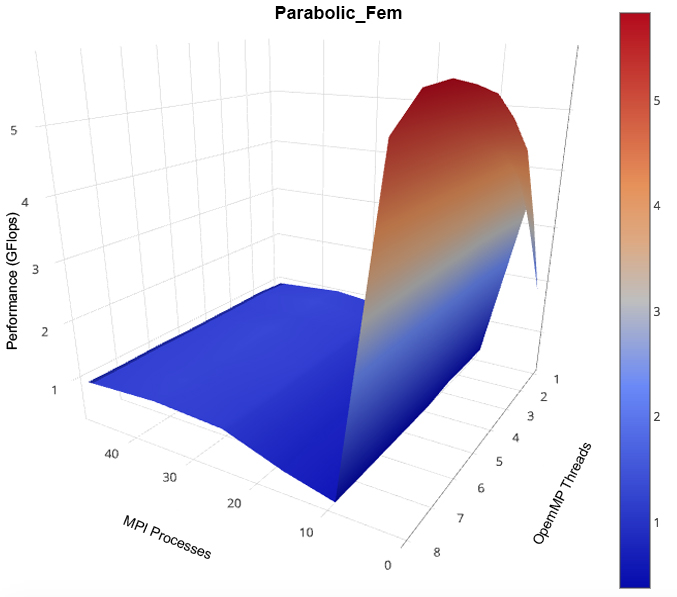
\includegraphics[scale=0.25]{figures/parabolicFem_surface.jpg}
		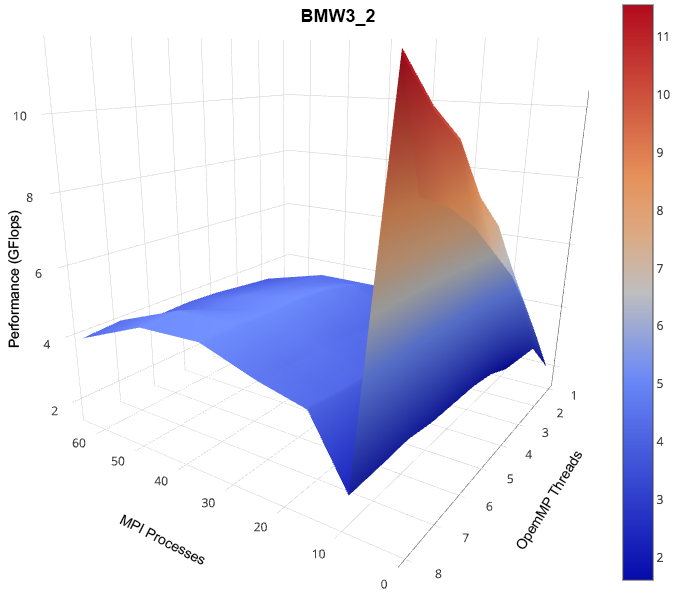
\includegraphics[scale=0.25]{figures/bmw3_2_surface.jpg}
		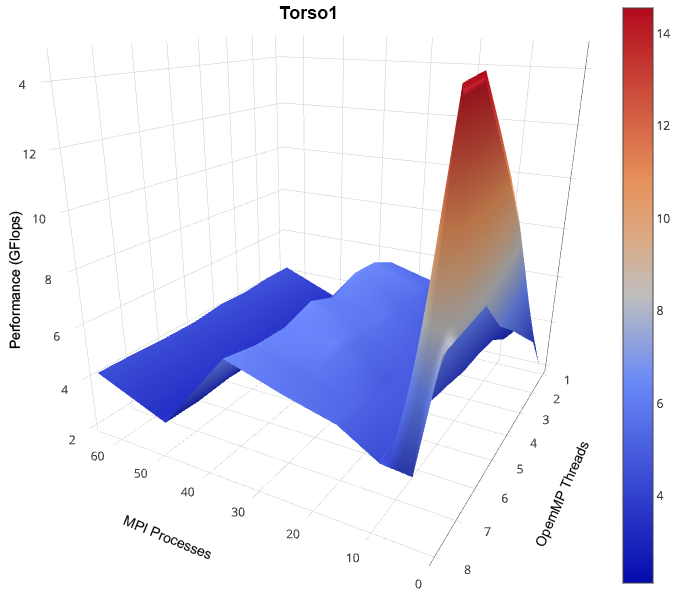
\includegraphics[scale=0.25]{figures/torso1_surface.jpg}
		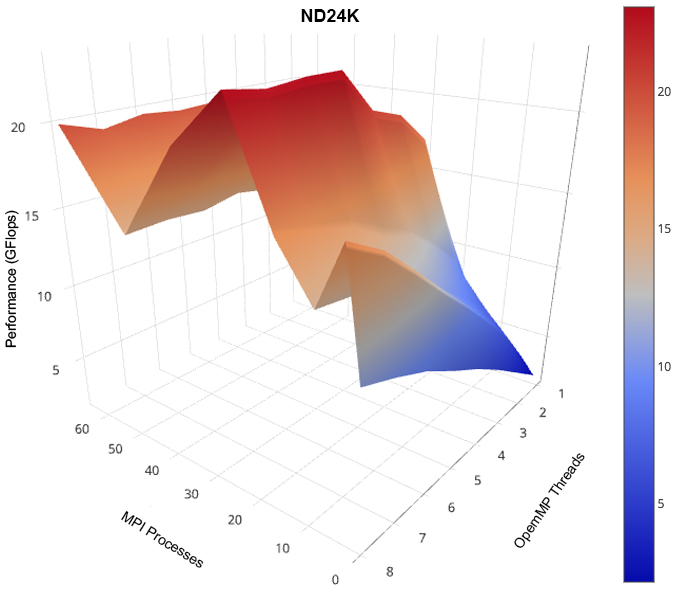
\includegraphics[scale=0.25]{figures/nd24k_surface.jpg}
		\caption{Hybrid SpMV Performance for Matrices with varying Sparsity}
		\label{fig:spmv-matrix-surfaces}
\end{centering}\end{figure*}

\begin{figure*}\begin{centering}
		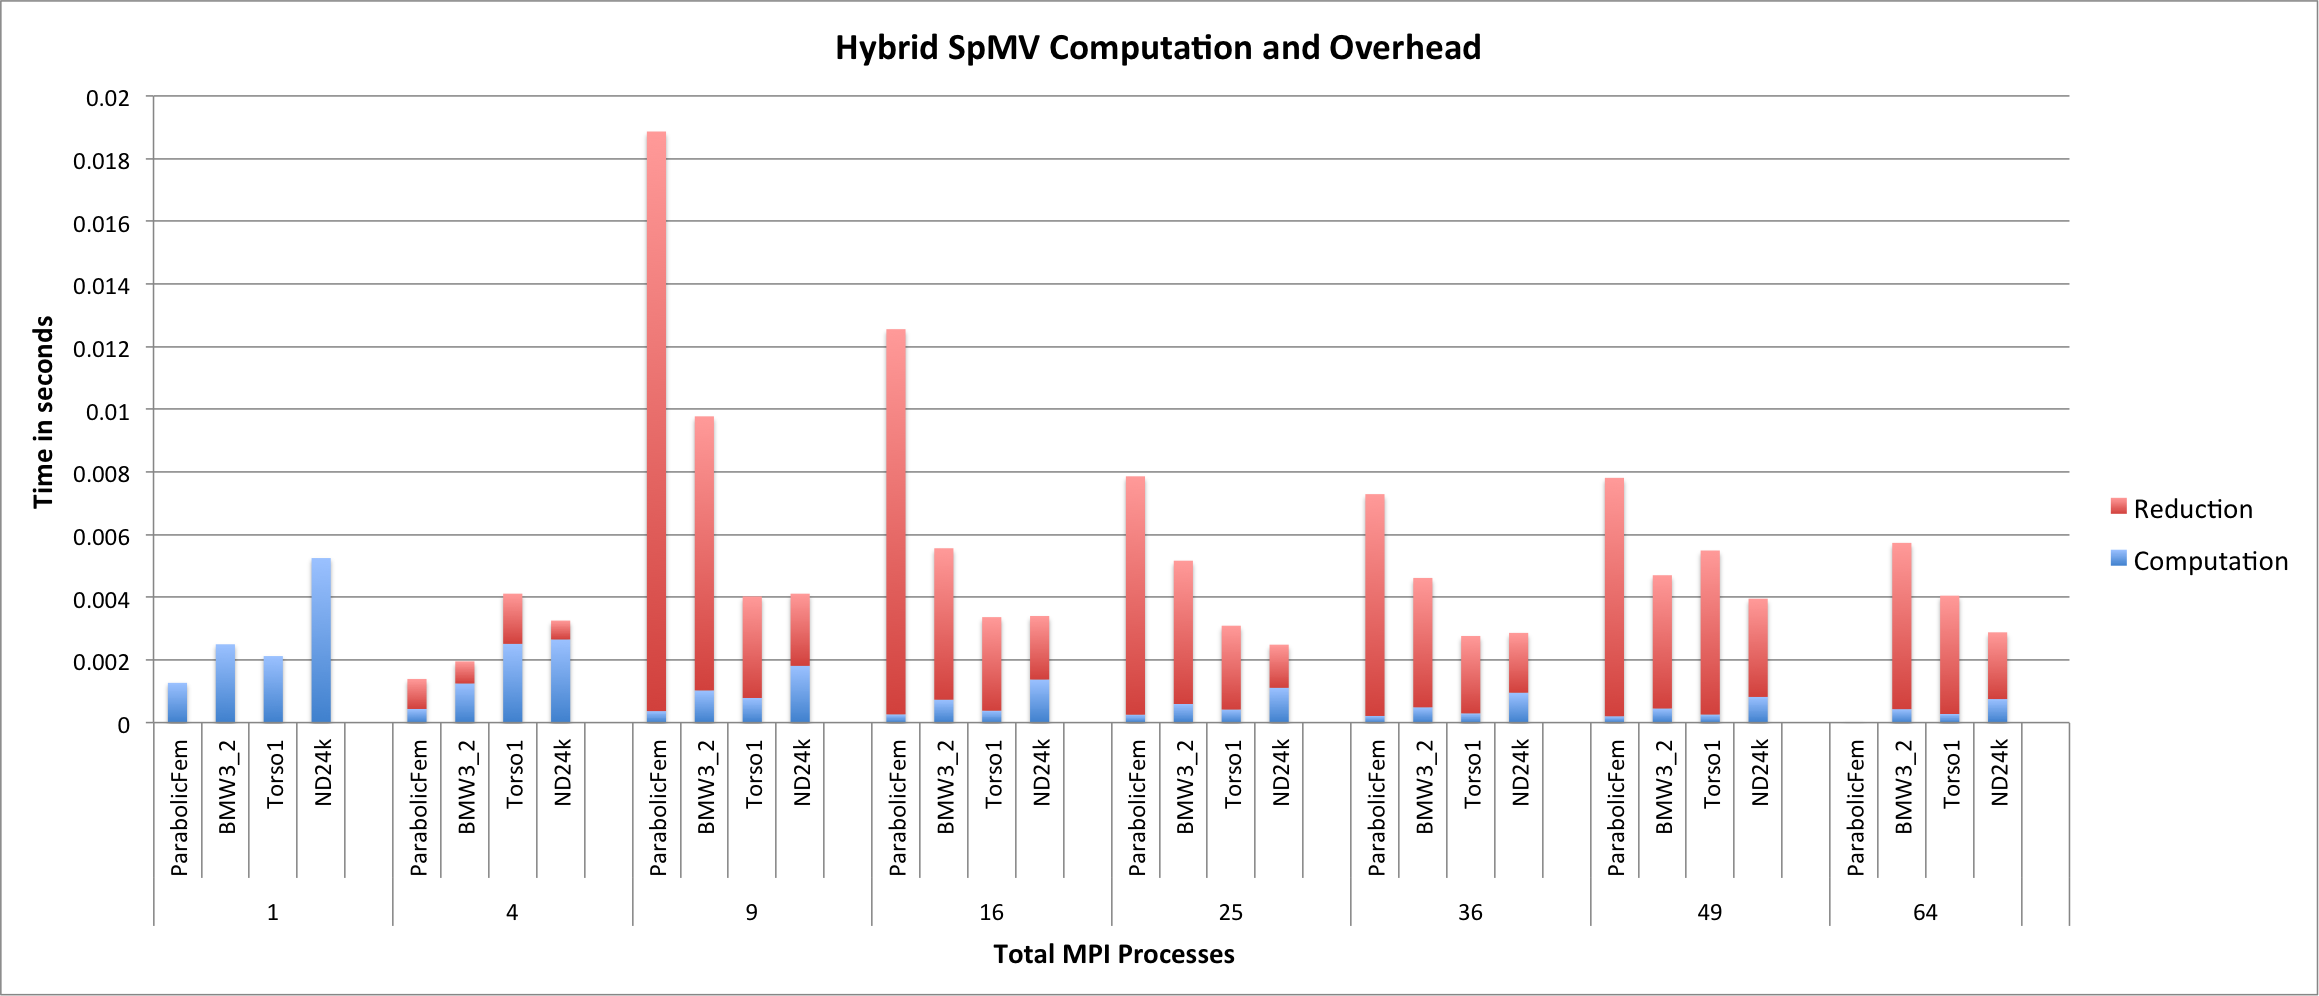
\includegraphics[scale=0.35]{figures/stackedbar_overhead.png}
		\caption{Computational Time and Reduce + Barrier Overhead}
		\label{fig:spmv-comp-and-reduction}
\end{centering}\end{figure*}

Increasing the number of processes eventually requires the use of additional nodes, thus introducing communication overhead.
We examined the performance impact of scaling up $p$ such that a node had between 1 and 16 processes. Subsequently we scaled thread count so that all available processing hardware on a node was used during the study. The performance characteristics for 2 MPI processes per node (where applicable) with varying total process count and threads per process are visible in Fig. \ref{fig:spmv-matrix-surfaces}. 

For all but the least sparse matrix performance accelerates quickly until 9-16 processes, followed by a sharp decline as overhead from the non-logarithmic \emph{MPI\_Reduce} outpaced the benefit of additional processes. These results agree with the analytical model from \ref{sec:spmv-analytic} where in such a decline is exhibited in Fig. \ref{fig:spmv-analytic-model}(a) for the Non-Overlapping case. Due to an inability to increase $p$ beyond 64 total processes ($8$x$8$ process matrix), our results did not indicate if nd24k would experience similar behavior, however, due to the impact sparsity has on performance at scale, it is likely that the trend exhibited in \ref{fig:spmv-analytic-model}(a) would hold true. 

	\subsection{Impact: Thread Count}\label{sec:dspmv-threadscaling}

\begin{figure}[H]
	\begin{centering}
		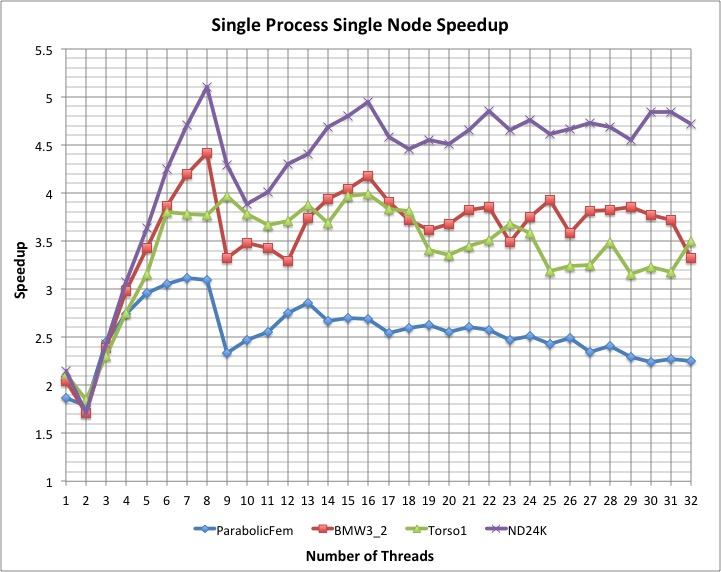
\includegraphics[scale=0.25]{figures/single_node_speedup.jpg}
		\caption{Single Node Speedup}
		\label{fig:spmv-page-singlenode}
\end{centering}
\end{figure}

Where computation is bound by memory references and cache hits capitalizing upon multi-core utilization can greatly increase performance \cite{blelloch2008provably}. In hybrid codes optimizing performance exhibited from a individual node is essential for overall execution. Figure \ref{fig:spmv-page-singlenode} illustrates the impact of increasing thread count locally on a single node due to the increased memory access as the socket cores become saturated with work. A peak can be seen near 8 threads with another visible peak at 16. 

Once all cores on a single processor are assigned a thread that chips memory bandwidth as been fully allocated thereby achieving the maximum on chip memory bandwidth. Beyond 8 threads an increase in overhead from the distribution of work amongst the disjoint memory profiles on each chip degrades performance until total memory bandwidth allocation overcomes this overhead. Over subscription of node sockets/cores produces stagnation and declines in speedup across all matrices examined. It is worth noting that the code generated for these experiments made no effort to control thread core or socket affinity, therefore it is highly likely that scheduling in an oversubscribed node is a cause for declining performance. 
	\subsection{Impact: Sparsity}\label{sec:dspmv-sparsityimpact}

The extent to which multi-core, mutli-node, or hybrid strategies are capable of producing increased performance is widely dependent on quantity and distribution of $nnz$ within a matrix. In the single process single node case, Fig. \ref{fig:spmv-page-singlenode}, only one the sub-matrix is created where $A_{ij} = A$. Given that the Algorithm \ref{alg:spmv} requires entire rows within a sub-matrix assigned to a process to be operated on by a single OpenMP thread, there is no decline in the $nnz$ per row. 

In contrast as the number of MPI processes is increased, $nnz$ per row within a sub-matrix $A_{ij}$ decreases proportionally to $p$. For example Parabolic\_Fem's initial $nnz$ per row of $~7$ when process count increases from 1 to 4, doubling the number of cols in the process matrix, and reduces $nnz$ per row  via $density_{A_{ij}}/p$. As can be seen in Fig. \ref{fig:spmv-matrix-surfaces} matrices with fewer $nnz$ per row, exhibit decline in multi-nodal performance more rapidly than those with greater initial starting $nnz$ pder row. In the case of Parabolic\_Fem, once $p > 6$ $nnz$ per row is less than 1, leading to work imbalances across processes and lost performance as a result. 

Subsequently while the average $nnz$ per row decreases quickly, overhead associated with reduction accross the larger process count in addition to the \emph{MPI\_Barrier} halting overall progress, begins to outpaced computation speedup seen from acquiring additional processes or nodes. Figure \ref{fig:spmv-comp-and-reduction} outlines that while computational time for SpMV may decrease, reduction and barrier weigh down overall run-times The gradual decrease in overhead seen is a symptom of decreased message size between each process and its $row master$, however a process with nothing to do will continue to have more overhead than productive computation. 





\section{Future Work}\label{sec:dspmv-futurework}
- run computation on larger number of nodes/cores
- wider range of sparsitys and non-zero distribution within matrices
- explore performance impact of different distribution/decomposition methods
- possible explore the impact of different storage formats within the different distribution methods
- gpus/knights landing

\section{Conclusions}\label{sec:sga-conclusion}




\bibliographystyle{IEEEtran}
\bibliography{dspmv-refs} 

\end{document}
